\section{Zielsetzung}
In diesem Versuch soll die Gültigkeit von Gleichung \ref{eqn:abbildung1}, \ref{eqn:abbildung2} und \ref{eqn:brenn1} überprüft werden, sowie die Funktionalität der Messmethoden von Bessel und von Abbe zur Brennweitenbestimmung.


\section{Theorie}
\label{sec:Theorie}
\subsection{Bildentstehung}
    \begin{figure}
        \centering
        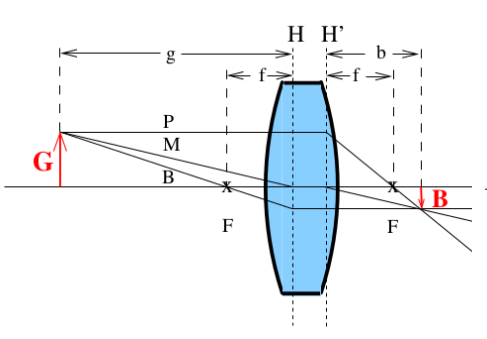
\includegraphics[width=10cm]{Bilder/veranschaulichung.png}
        \caption{Abgebildet ist die schematische Bildentstehung durch eine Sammellinse.}
        \label{fig:veranschaulichung}
    \end{figure}

    \noindent Die Größe eines scharfen Bildes auf einem Schirm ist zunächst über die drei Geraden $P$, $M$ und $B'$ bestimmt, welche in \ref{fig:veranschaulichung} dargestellt sind. $P$ beshreibt hierbei die Strahlen, die Parallel zu der Verbindungsachse
    zwischen dem Gegenstand $G$ und dem Bild $B$ verläuft und $B'$ der Brennpunktstrahl. Nachdem der erste Parallelstrahl an der zweiten Hauptebene $H'$ gebrochen wird, wird dieser zum Brennpunktstrahl und der erste Brennpunktstrahl wird an der ersten
    Hauptebene zu einem Parallelstrahl gebrochen. $M$ verläuft dabei zwischen den beiden Strahlen und wird an beiden Hauptebenen gebrochen, sodass er zwischen diesen auf der Verbindungsachse liegt und hinter $H'$ die gleiche Steigung hat, wie vor $H$.
    Die Schnittpunkte der Geraden $P$ und $B'$ mit der Verbindungsachse zwischen $G$ und $B$ gibt dann die Brennweite der Linse.

\subsection{Eigenschaften scharfer Bilder}
    \noindent Bei Linsen wird generell zwischen Sammellinsen und Zerstreuungslinsen unterschieden. Sammel und Streuungslinsen unterscheiden sich dadrin, dass die Brennweite $f$ bei Sammellinsen positiv ist und bei Zerstreuungslinsen negativ.
    Zusätzlich werden auch zwei Hauptebenen definiert, an denen die Brechung mathematisch modelliert wird. Im Fall einer dünnen Linse fallen die beiden Hauptebenen auf die Mittelebene zusammen. Der Abbildungsmaßstab $V$, der das Verhältnis der Bildgröße $B$
    zu der Gegenstandsgröße $G$ wiedergibt, wird in diesem Fall auch zu
    \begin{equation}
        V=\frac{B}{G} 
        \label{eqn:abbildung1}
    \end{equation}
    \begin{equation}
        V=\frac{b}{g} \text{,}
        \label{eqn:abbildung2}
    \end{equation}
    \noindent wobei $b$ der Abstand zwischen dem Bild und der Mittelebene ist und $g$ der Abstand vom Gegenstand zur Mittelebene.
    Des weiteren gilt bei solchen Linsen für die Brennweite die Beziehung
    \begin{equation}
        f=\frac{bg}{b+g} \text{,}
        \label{eqn:brenn1}
    \end{equation}
    \noindent wenn das Bild in der Bildebene scharf erscheint.

    \noindent Für den Fall, dass mit zwei Linsen gearbeitet wird, wobei eine eine Sammellinse und eine eine Streulinse ist, ist es möglich, falls beide dünn genug sind, für beide Linsen zwei gemeinsame Hauptebenen zu definieren.
    Dazu wird im Aufbau ein Referenzpunkt A gewählt, dessen Abstand zum Gegenstand $g'$ und zum Bildschirm $b'$ über die beiden Gleichungen
    \begin{align}
       & g'=f(1+\frac{1}{V})+h \\
        & b'=f(1+V)+h'
        \label{eqn:abbe}
    \end{align}
    bestimmt sind, wobei $h$ der Abstand von $A$ zur Hauptebene $H$ ist und $h'$ der Abstand von $A$ zur anderen Hauptebene $H'$.
\subsection{Abberration}
    \noindent Ein Effekt der bei Linsen auftritt, der beachtet werden muss, ist die chromatische Abberration. Diese beschreibt eine Verzerrung des Bildes, dessen Licht durch eine Linse läuft. Diese tritt auf aufgrund der verschiedenen Wellenlängen, die unterschiedlich gebrochen werden an dieser.
    Als Folge entstehen bei nicht monochromatischem Licht mehrere Bilder auf dem Schirm, die unterschiedlichen Wellenlängen entsprechen und somit die Präzision von Messungen an dem Bild verschlechtert werden. Des weiteren kann spärische Aberration auftreten, dadurch,
    dass Lichtstrahlen stärker an den Rändern einer sphärischen Linse gebrochen werden, als am Rand, welches das Bild weiter unschärfer macht.

    \noindent Die Brechkraft
    \begin{equation}
        \label{eqn:Brechkraft}
        D=\frac{1}{f}
    \end{equation}
    eines Linsensystems kann durch
    \begin{equation}
        D=\sum_i^N{D_i}
        \label{eqn:Brechkraft2}
    \end{equation}
    berechnet werden.

    \cite{V408}

